%
% File acl2012.tex
%
% Contact: gdzhou@suda.edu.cn
%%
%% Based on the style files for ACL2008 by Joakim Nivre and Noah Smith
%% and that of ACL2010 by Jing-Shin Chang and Philipp Koehn


\documentclass[11pt]{article}
\usepackage{acl2012}
\usepackage{times}
\usepackage{latexsym}
\usepackage{amsmath}
\usepackage{multirow}
\usepackage{url}
\usepackage{graphicx}
\DeclareMathOperator*{\argmax}{arg\,max}
\setlength\titlebox{6.5cm}    % Expanding the titlebox

\title{Multilabels for Annotation of Word Sense}

\author{First Author \\
   Affiliation / Address line 1 \\
   Affiliation / Address line 2 \\
   Affiliation / Address line 3 \\
  {\tt email@domain} \\\And
   Second Author \\
   Affiliation / Address line 1 \\
   Affiliation / Address line 2 \\
   Affiliation / Address line 3 \\
   {\tt email@domain} 
\\}

\date{}


\begin{document}
\maketitle
\begin{abstract}

\end{abstract}

\section{Introduction} % 1.0 page

Much NLP annotation involves categorical distinctions of phenomena
that can be defined by example or by description, although the
linguistic facts that correlate with the category distinctions remain
to be discovered. Annotation guidelines are constructed in order to
train annotators in the the annotation category definitions and
examples. The annotators’ role is to annotate language data in order
to make the categorical distinctions explicit. When annotation is
performed reliabily by different annotators, the annotated data
supports the research needed for discovery and analysis of the
linguistic correlates of a phenomenon of interest. 

However, many semantic and pragmatic dimensions of language use that
are relevant or even important to capture are either clearly not
categorical, or categorization is difficult due to a set of categories
that is too numerous, too interdependent, or too fluid. 

In addition, it is costly to train annotators, and the use the trained
annotators for to label data. We address a word sense annotation
procedure in which the sense labels are relatively numerous and
potentially interdependent, and where we assume that in some cases an
instance of a word in context can evoke a novel sense reading
\cite{ludlow2005}.

Our data consists of multilabels for each word sense instance, where
the multilabel for each in- stance consists of a set of labels, each
provided by a different annotator. Collecting multilabels for each
instance provides much greater dimensionality to the agreement or
disagreement among annotators on a given instance, thus highlighting
that disagreement has many gradations.

In previous work, we have argued that interannotator agreement on many
word instances by the same annotators indicates that the trained
annotators can perform the general procedure reliably.  Even so, the
agreement among trained annotators can still be low for a particular
word instance.  

In other previous work, we compared performance of an unsupervised
learning method to learn an unknown (hidden) {\it true} label from
multilabels of different sizes, and where the labelers were trained or
not. 

In separate work on multilabel annotation with multiple labelers, we
showed the use of a hierarchical Bayesian model of annotation to
estimate annotator accuracy and bias along with item difficulty from
the observed sets of multilabels. Here we will build on both lines of
investigation to compare different estimates of annotator accuracy. We
also examine other sources of uncertainty regarding word sense
multilabels, such as item difficulty.

\section{Related Work} % 0.25 page

Multilabels have been used in epidemiology and more recently in
machine learning for the problem of reducing the cost of label
acquisition, or improving label accuracy of manual labels, or
both~\cite{dawidSkene79,snowEtAl08,shengEtAl_2008}. For this type of
multilabel, it is assumed that there is a true label and that each
annotator who contributes to a multilabel for each instance has an
unknown probability of being correct that is (sometimes much) less
than 100\%.  Furthermore, error patterns are characterized directly.

Multilabels of a very different sort have also been used in machine
learning approaches to address the problem of how to assign instances
to multiple
classes~\cite{tsoumakas&katakis_2007,boutellEtAl_2004,mccallum_1999}.
The assumption behind these approaches is that there are instances
that cannot be assigned a single label because they belong partly to
one class and partly to another. For a multilabel to represent
simultaneous membership of an instance in multiple classes, each class
represented in the multilabel should be a {\it true} class.  For
example, a news article about the steroid scandal in American baseball
making it to the U.~S.~Congress might be classified as being about
sports and about politics.

With word senses, a given word may seem to have properties of more
than one sense in a given sense inventory, in which case a multilabel
can represent all the senses the word exhibits. 
% give examples from LRE paper for 'fair' and 'quiet'.

Word meaning has been variously represented in lexicography,
linguistics and computational linguistics. Approaches include a
hierarchy of sense definitions (as in conventional dictionaries),
WordNet's ordered inventory of sets of synonyms plus sense
definitions~\cite{millerEtAl93}, one or more components of a
conceptual frame as in FrameNet~\cite{fillmoreEtAl03}, a decomposition
into logical predicates and operators~\cite{dowty79}, a cluster of
sentences where a word form in all of them has the same meaning (as
argued for in~\cite{kilgarriff97}), or some combination of the above.
Recent work by Erk and colleagues builds on the view that a sense can
be defined as the contexts it occurs in~\cite{kilgarriff97}, or more
specifically as regions in a vector space model~\cite{erk09}. 

We rely on WordNet senses for our annotation tasks. Since all
sentences for a given lemma are annotated at the same time, and the
WordNet senses include glosses along with definitions, our annotation
task is similar to clustering instances by their similarity to the
glosses.

\begin{figure}
\begin{center}
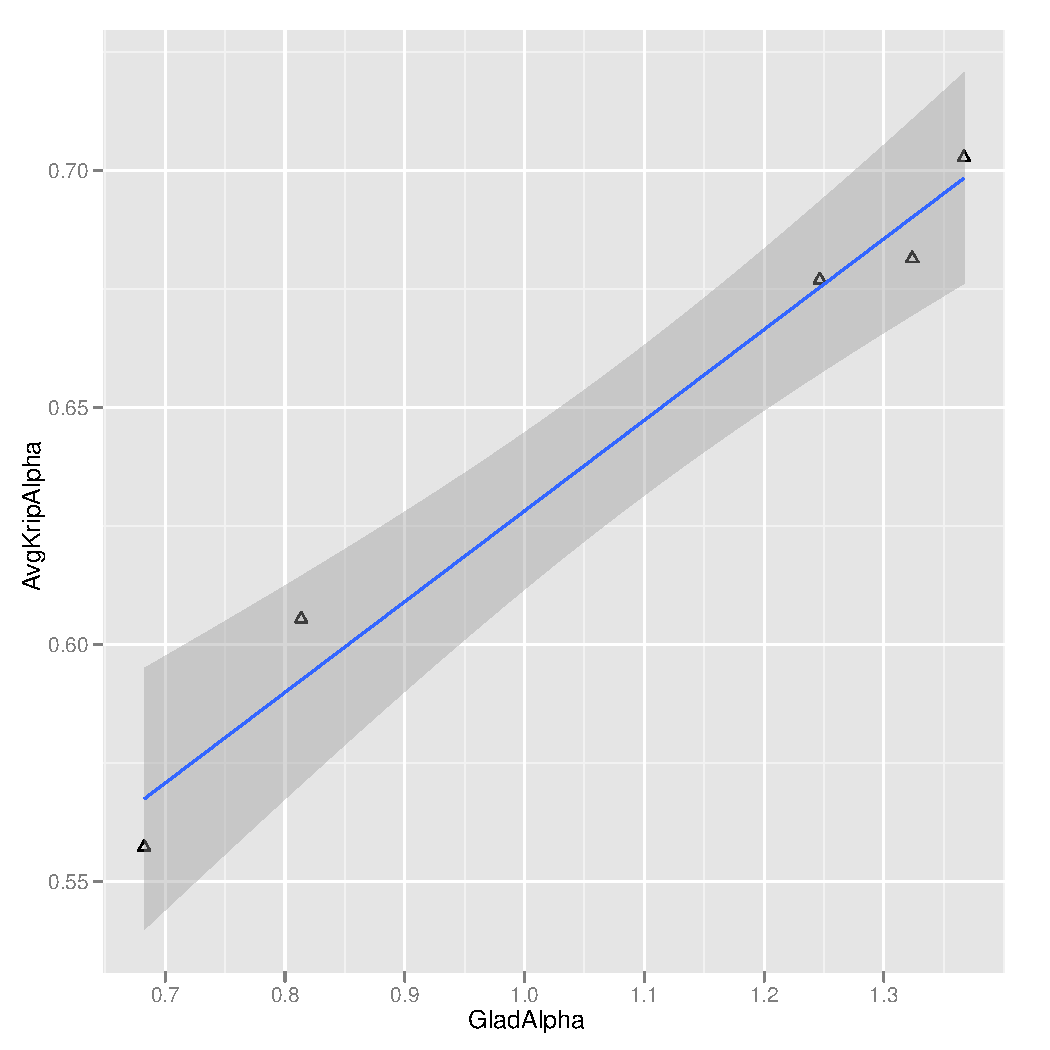
\includegraphics[width=0.4\textwidth]{img/GladVsKripp.pdf}
\end{center}
\caption{Average Krippendorf $\alpha$ versus GLAD $\alpha$
  (logit-scaled probability of correct responsse) for five trained annotators
  over 99 instances of the word {\it fair}.  The line and error band is for a
  linear regression fit.}\label{glad-alpha.fig}
\end{figure}
%  
\begin{figure*}[ht]
\includegraphics[width=\textwidth]{img/fair-response.pdf}
\caption{Estimated annotator response to given categorical inputs.
  Each block repreents a different annotator.  Each row represents a
  given true label and each column represents a possible response by
  an annotator, with the shading performed by coloring on the logit
  scale ($\mbox{logit}(\theta) = \log
  \theta/(1-\theta)$).}\label{dawid-skene.fig}
\end{figure*}


\section{Word Sense and Multilabels} % 0.5 page

WordNet is a large lexical resource that has been used for a
large-scale word sense annotation project as part of a project to
create a Manually Annotated SubCorpus (MASC) of the Open American
National Corpus (OANC)~\cite{ideEtAl10}. The word sense corpus,
described more fully in ~\cite{passonneauEtAl12}, consists of a
sentence corpus from MASC (and supplemented where needed from the OANC
for more lower frequency words) with approximately 1,000 sentences
each for 100 words representing nouns, verbs and adjectives. All
instances of the 100 words have been annotated with WordNet senses.
The average number of WordNet senses is approximately 8 per word. For
each word, about 900 instances were annotated by a single annotator
from a pool of 10 trained annotators, and the remaining 100 by four
annotators. We have 10 words that were annotated by six trained
annotators, and 3 words additionally annotated by 14 Mechanical
Turkers.%
%
\footnote{Mechanical Turk is a service provided by Amazon, Inc.,
wherein workers can be hired to fill in web-based forms, which can
be used for annotation.  See {\tt https://www.mturk.com/mturk/welcome}.}
%
We use this sample of 1000 instances to illustrate the
Bayesian model for estimating annotator quality and true labels.

\section{Annotator Quality and Multilabels} % 1 page

Much work on annotation measures reliability of annotators, meaning
their consistency on the annotation task, using pairwise agreement or
an agreement coefficient such as $\kappa$~\cite{cohen60} or
$\alpha$~\cite{krippendorff80}. These metrics cannot rank annotators
by their quality, they can only be used to rank annotators by their
level of agreement with other annotators.  These metrics also do
not provide item-by-item true label judgements nor do they predict
the accuracy of a corpus with a given level of agreement.

Annotator quality as estimated by statistical models such as
GLAD~\cite{dawidSkene79,whitehillEtAl-2009} differs from measures of
interannotator agreement in that they provide accuracy and bias
estimates for each annotator as well as probabilistic labels for each
item in the corpus (i.e., estimating that a given word has a 93\%
chance of being sense 1 and a 7\% chance of being sense 2, or that a
given annotator has an 81\% chance of returning sense 1 for a word
truly of sense 1 and a 15\% chance of returning sense 2 and a 4\%
chance of returning sense 3).

As shown in Figure~\ref{glad-alpha.fig}, we find a correlation of
average interannotator agreement and GLAD annotator quality scores on
some senses.  Note in particular that the ranking of annotators
is the same.  In part, this is because GLAD-like models estimate
the true category using an adjustment to voting-based estimates
as reflected in average Krippendorf-$\alpha$ using annotator
accuracies.

A drawback to using GLAD for multilabels is that it is only defined
for binary annotations.  Thus we need to decompose the multilabels
in a sequence of unrelated binary labeling problems, which loses
the structural information that each annotator only provides one
label.  

Instead, we will follow \cite{dawidSkene1979} in treating responses as
multinomial.  In this setting, each annotator is described by a
response matrix, which is like a probabilistically scaled confusion
matrix. This matrix indicates which response is likely from the
annotator for an item of a given input category.  An example is shown
in Figure~\ref{dawid-skene.fig}.
%

% \section{Item Difficulty and Multilabels}


% \section{Conclusion} % 0.25 page

% \section*{Acknowledgments}

\cleardoublepage
\bibliographystyle{acl2012}
\bibliography{wordsense-multilabels}
\end{document}
